\let\negmedspace\undefined
\let\negthickspace\undefined
\documentclass[journal,12pt,onecolumn]{IEEEtran}
\usepackage{cite}
\usepackage{amsmath,amssymb,amsfonts,amsthm}
\usepackage{algorithmic}
\usepackage{graphicx}
\graphicspath{{./figs/}}
\usepackage{textcomp}
\usepackage{xcolor}
\usepackage{txfonts}
\usepackage{listings}
\usepackage{enumitem}
\usepackage{mathtools}
\usepackage{gensymb}
\usepackage{comment}
\usepackage{caption}
\usepackage[breaklinks=true]{hyperref}
\usepackage{tkz-euclide} 
\usepackage{listings}
\usepackage{gvv}                                        
%\def\inputGnumericTable{}                                 
\usepackage[latin1]{inputenc}     
\usepackage{xparse}
\usepackage{color}                                            
\usepackage{array}                                            
\usepackage{longtable}                                       
\usepackage{calc}                                             
\usepackage{multirow}
\usepackage{multicol}
\usepackage{hhline}                                           
\usepackage{ifthen}                                           
\usepackage{lscape}
\usepackage{tabularx}
\usepackage{array}
\usepackage{float}
%\newtheorem{theorem}{Theorem}[section]
%\newtheorem{theorem}{Theorem}[section]
%\newtheorem{problem}{Problem}
%\newtheorem{proposition}{Proposition}[section]
%\newtheorem{lemma}{Lemma}[section]
%\newtheorem{corollary}[theorem]{Corollary}
%\newtheorem{example}{Example}[section]
%\newtheorem{definition}[problem]{Definition}

\begin{document}

\title{4.13.23}
\author{EE25BTECH11018 - Darisy Sreetej}
% \maketitle
% \newpage
% \bigskip
%\begin{document}
{\let\newpage\relax\maketitle}
%\renewcommand{\thefigure}{\theenumi}
%\renewcommand{\thetable}{\theenumi}
\textbf{Question:}\\
Let $a, b, c ,d$ be non-zero numbers. If the point of intersection of the lines $4a\vec{x} +2a\vec{y} + c = 0$ and $5b\vec{x} + 2b\vec{y} + d = 0$ lies in the fourth quadrant and is equidistant from the two axes then
\begin{enumerate}
    \item $3bc-2ad=0$
    \item $2bc-3ad=0$
    \item $3bc+2ad=0$
    \item $2bc+3ad=0$
\end{enumerate}
\solution\\
The two lines are
\begin{align}
4a\vec{x} +2a\vec{y} + c = 0  , \\
5b\vec{x} + 2b\vec{y} + d = 0 
\end{align}
According to the condition,the intersection point is equidistant from the axes and lies in the fourth quadrant, so its coordinates satisfy $y=-x$ \\
\begin{align}
\vec{x}+\vec{y}=0
\end{align}
This equation can be expressed in terms of matrices
\begin{align}
\myvec{4a\\2a}^\top\myvec{\vec{x}\\\vec{y}}=-c\\
\myvec{5b\\2b}^\top\myvec{\vec{x}\\\vec{y}}=-d\\
\myvec{1\\1}^\top\myvec{\vec{x}\\\vec{y}}=0
\end{align}
They can be represented as,
\begin{align}
    \myvec{4a&5b\\2a&2b\\1&1}^\top\myvec{\vec{x}\\\vec{y}}=\myvec{-c\\-d\\0}
\end{align}
Using augmented matrix,
\begin{align}
\augvec{2}{1}{4a&2a&-c\\5b&2b&-d\\1&1&0}
\end{align}
$R_3=R_3-4aR_1$\\
$R_2=R_2-5bR_1$
\begin{align}
\augvec{2}{1}{1&1&0\\0&-3b&-d\\0&-2a&-c}
\end{align}
$R_3=R_3-\frac{2a}{3b}R_2$
\begin{align}
\augvec{2}{1}{1&1&0\\0&-3b&-d\\0&0&-c+\frac{2ad}{3b}}
\end{align}
\begin{align}
\augvec{2}{1}{1&1&0\\0&-3b&-d\\0&0&\frac{2ad-3bc}{3b}}
\end{align}
The last row of the matrix represents the equation
\begin{align}
\vec{y}0+\vec{x}0=\frac{2ad-3bc}{3b}
\end{align}
For the system to be consistent(i.e., to have a solution),the right-hand side must be zero.
\begin{align}
\frac{2ad-3bc}{3b}=0
\end{align}
\begin{align}
2ad-3bc=0
\end{align}
Therefore,
\begin{align}
3bc=2ad
\end{align}
Therefore, option(a) is correct\\
For the point of intersection , solve the equations from (11),\\
The point of intersection is 
\begin{align}
    \myvec{\vec{x}\\\vec{y}}=\myvec{\frac{-d}{3b}\\\frac{d}{3b}}
\end{align}
Also ,
\begin{align}
 \myvec{\vec{x}\\\vec{y}}=\myvec{\frac{-c}{2a}\\\frac{c}{2a}}  \quad (from (15))
\end{align}
\begin{figure}[h!]
    \centering
    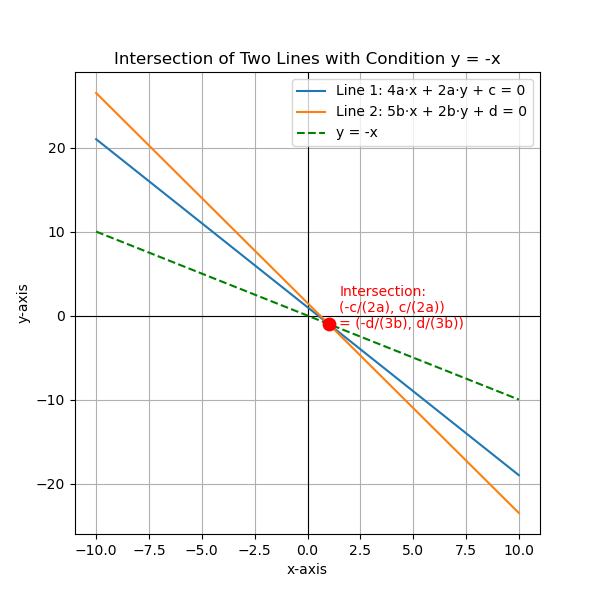
\includegraphics[height=0.5\textheight, keepaspectratio]{figs/fig.png}
    \label{figure_1}
\end{figure}
\end{document}

